\begin{figure}[hbtp]
  \centering
  \subfigure{
    \label{fig:8020-affected--all}
    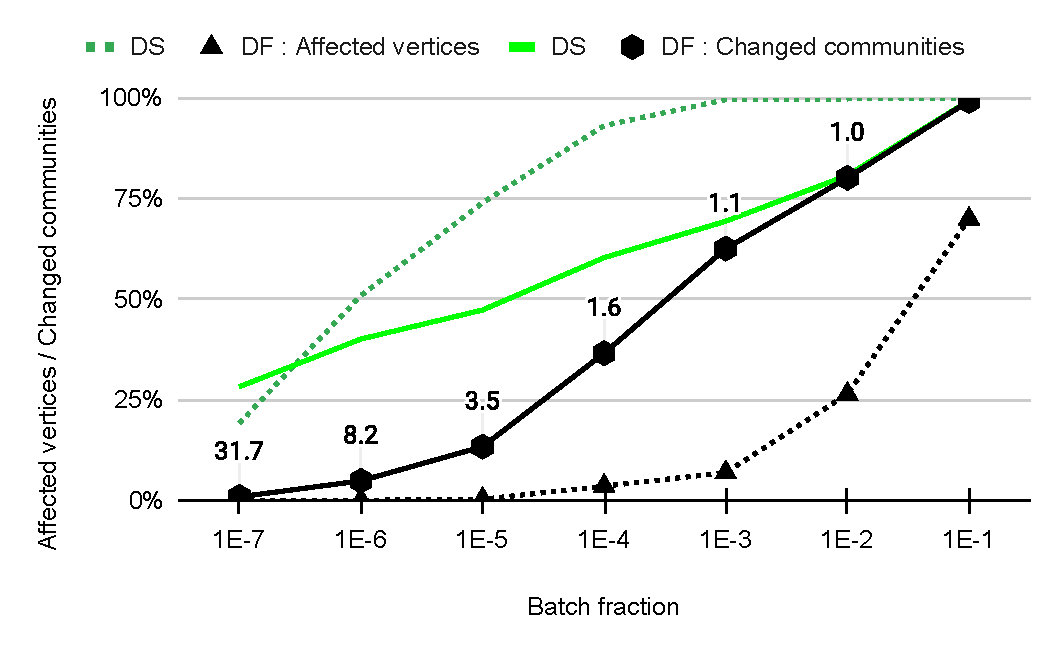
\includegraphics[width=0.85\linewidth]{out/8020-affected.pdf}
  } \\[-1ex]
  \caption{Fraction of vertices marked as affected (average) with \textit{Delta-screening (DS)} and \textit{Dynamic Frontier (DF) Leiden} on graphs in Table \ref{tab:dataset-large}. The labels indicate the ratio of vertices identified as affected by DS Leiden to that of DF Leiden \su{TO}.}
  \label{fig:8020-affected}
\end{figure}
